\documentclass[12pt,a4paper,titlepage]{article}

\usepackage{preamble}

\title{Semantic Segmentation with Deep Learning}
\author{Saâd Aziz Alaoui, Yassine Jamoud, Samy Haffoudhi}
\date{\today}

\begin{document}

\maketitle

\section*{Introduction}

Le TP suivant porte sur de l'utilisation de techniques de Deep Learning pour la segmentation
sémantique. Cette dernière consiste à étiqueter chaque pixel d’une image avec une classe
correspondante à ce qui est représenté. L'idée derrière l'utilisation de Deep Learning est que
les outils automatiques permettent de gagner énormément de temps et d'argent pour les diagnostics
biomédicaux, ces outils deviennent de plus en plus cruciaux car les machines peuvent épauler
les analyses effectuées par les radiologues, afin de réduire le temps nécessaire pour établir
des diagnostics. Nous nous intéressons ici à l'architecture \textbf{U-Net} qui permet justement d'effectuer
des taches de segmentation sémantique. Le U-net est un réseau de neurones à convolution entièrement
convolutionnel. L'idée principale derrière cette architecture est de remplacer les opérations
de pooling par des opérateurs de suréchantillonnage ce qui implique l'augmentation de de la
résolution de la sortie. Nous verrons lors de ce TP les différents atouts et défauts que comporte
cette architecture en l'appliquant à des images biomédicales.

\section{Les données}

Nous disposons pour ce TP de différentes images biomédicales et plus précisément, des
images de cellules. Ces données sont regroupées entre un dossier de test et un dossier
d'entrainement. On dispose, pour les images d'entrainement, de plusieurs images qui, un
fois combinées, correspondent au masque.

\begin{figure}[H]
    \caption{Un exemple d'image et du masque associé}
    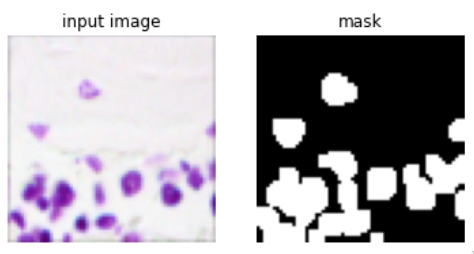
\includegraphics[width=0.6\textwidth]{exemple_image}
    \centering
\end{figure}

Nous disposons de 50 images pour l'entrainement. On les sous-échantillonne toutes
au mêmes dimensions et on conserve uniquement les 3 premiers canaux. De même pour
les labels mais on dispose que d'un unique canal.

\section{Le modèle}

\subsection{L'architecture}

Le modèle u-net est composé d'une couche d'entrée, un encodeur et un décodeur.
L'encodeur et le décodeur ont une structure en blocs similaires mais des dimensions différentes.
Chaque bloc de l'encodeur est composé de deux couches de convolution de mêmes dimensions,
d'une couche de pooling et d'une fonction d'activation. Pour compenser la baisse de la
dimension de l'image, le nombre de filtres augmente. Enfin, le modèle dispose également d'une
liste de connexions entre l'encodeur et le décodeur.

Une visualisation de l'architecture est disponible en annexe A. On observe bien la forme en U.

\subsection{Les fonctions de coût}

Le coefficient de Dice vaut $s = \frac{2 \lvert X \cap Y \rvert}{\lvert X \rvert + \lvert Y \rvert}$.
Cet indice permet de mesurer la similarité entre deux ensembles $X$ et $Y$. IL varie de
0 quand X et Y sont disjoints à 1 quand X et Y sont égaux.

La fonction de coût Dice est alors définie par $L(y_{pred}, y_{true}) = 1 - s(y_{pred}, y_{true})$.

\section{Entrainement et test}

Pour entrainer le modèle on utilise 25 epochs et un batch size de 25.

On remarque naturellement l'impact des dimensions des images. Plus ces dernières sont
grandes, plus l'entrainement est long. Par exemple, pour notre machine on obtient comme temps
d'éxécution :

\begin{itemize}
    \item{0.6s par step pour des images de taille (64, 64)}
    \item{8s par step pour des images de taille (256, 256)}
\end{itemize}

On obtient les tracés suivants :

\begin{figure}[H]
    \caption{Accuracy \& Loss}
    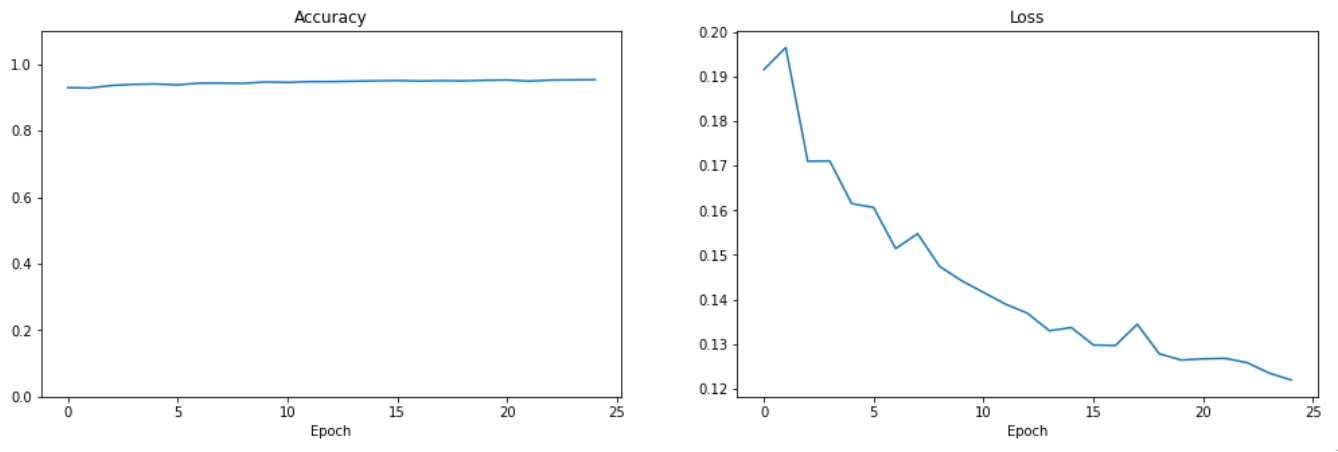
\includegraphics[width=\textwidth]{train}
    \centering
\end{figure}

\begin{appendices}

    \section{Architecture du modèle}

    \begin{figure}[H]
        \caption{Architecture du modèle}
        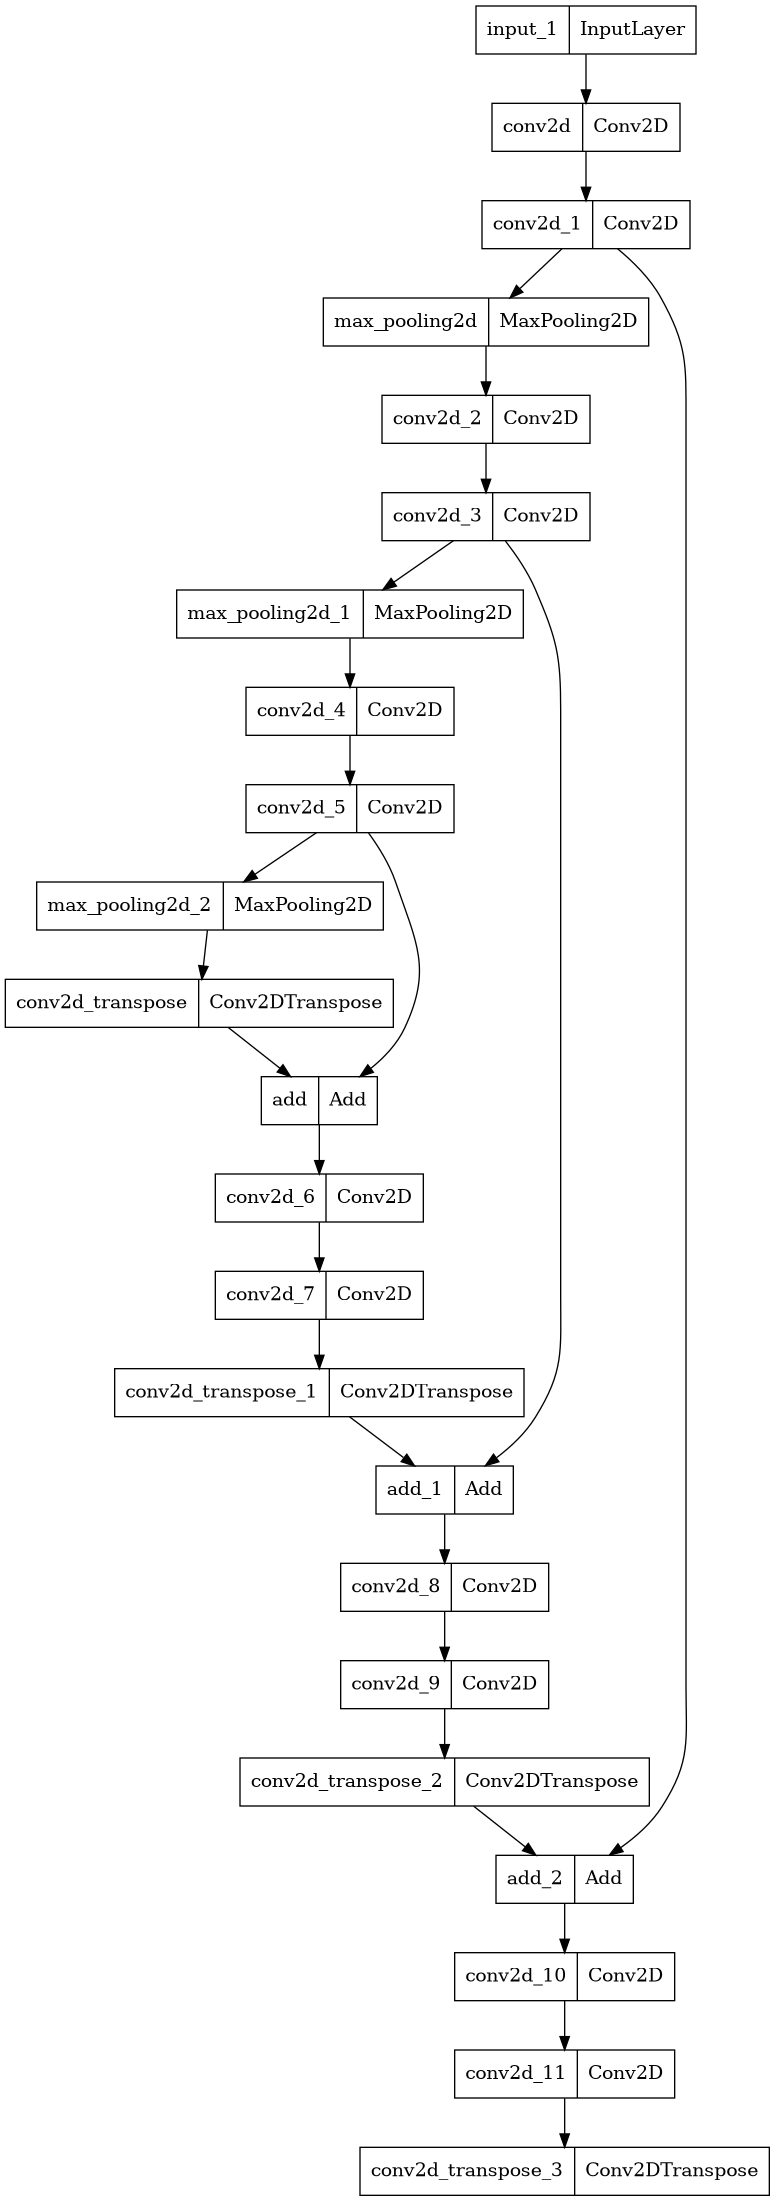
\includegraphics[width=0.4\textwidth]{model}
        \centering
    \end{figure}

\end{appendices}

\end{document}
